\section{Results}
\label{sec:results}

The pipeline converted the four public camera views into structured detection
records and annotated output videos. Across the evaluated run, the system
produced 17,117 person detections across 2,400 frames with detections. These
detections were organized into 358 per-camera tracks and 351 global
pseudonymous profiles. Seven global profiles appeared in more than one camera
view, and seven detections included an explicit cross-camera match score.

\subsection{Observation Volume}
\label{subsec:observation-volume}

Figure~\ref{fig:detection-volume} summarizes the number of person detections,
per-camera tracks, and global pseudonymous profiles by camera view. The result
shows that the raw video feeds can be converted into a large set of structured
records. In the context of the research question, this figure establishes the
first step of the privacy-relevant process: public video is not only viewable by
humans, but can also be transformed into machine-readable observation data.

\begin{figure}[htbp]
    \centering
    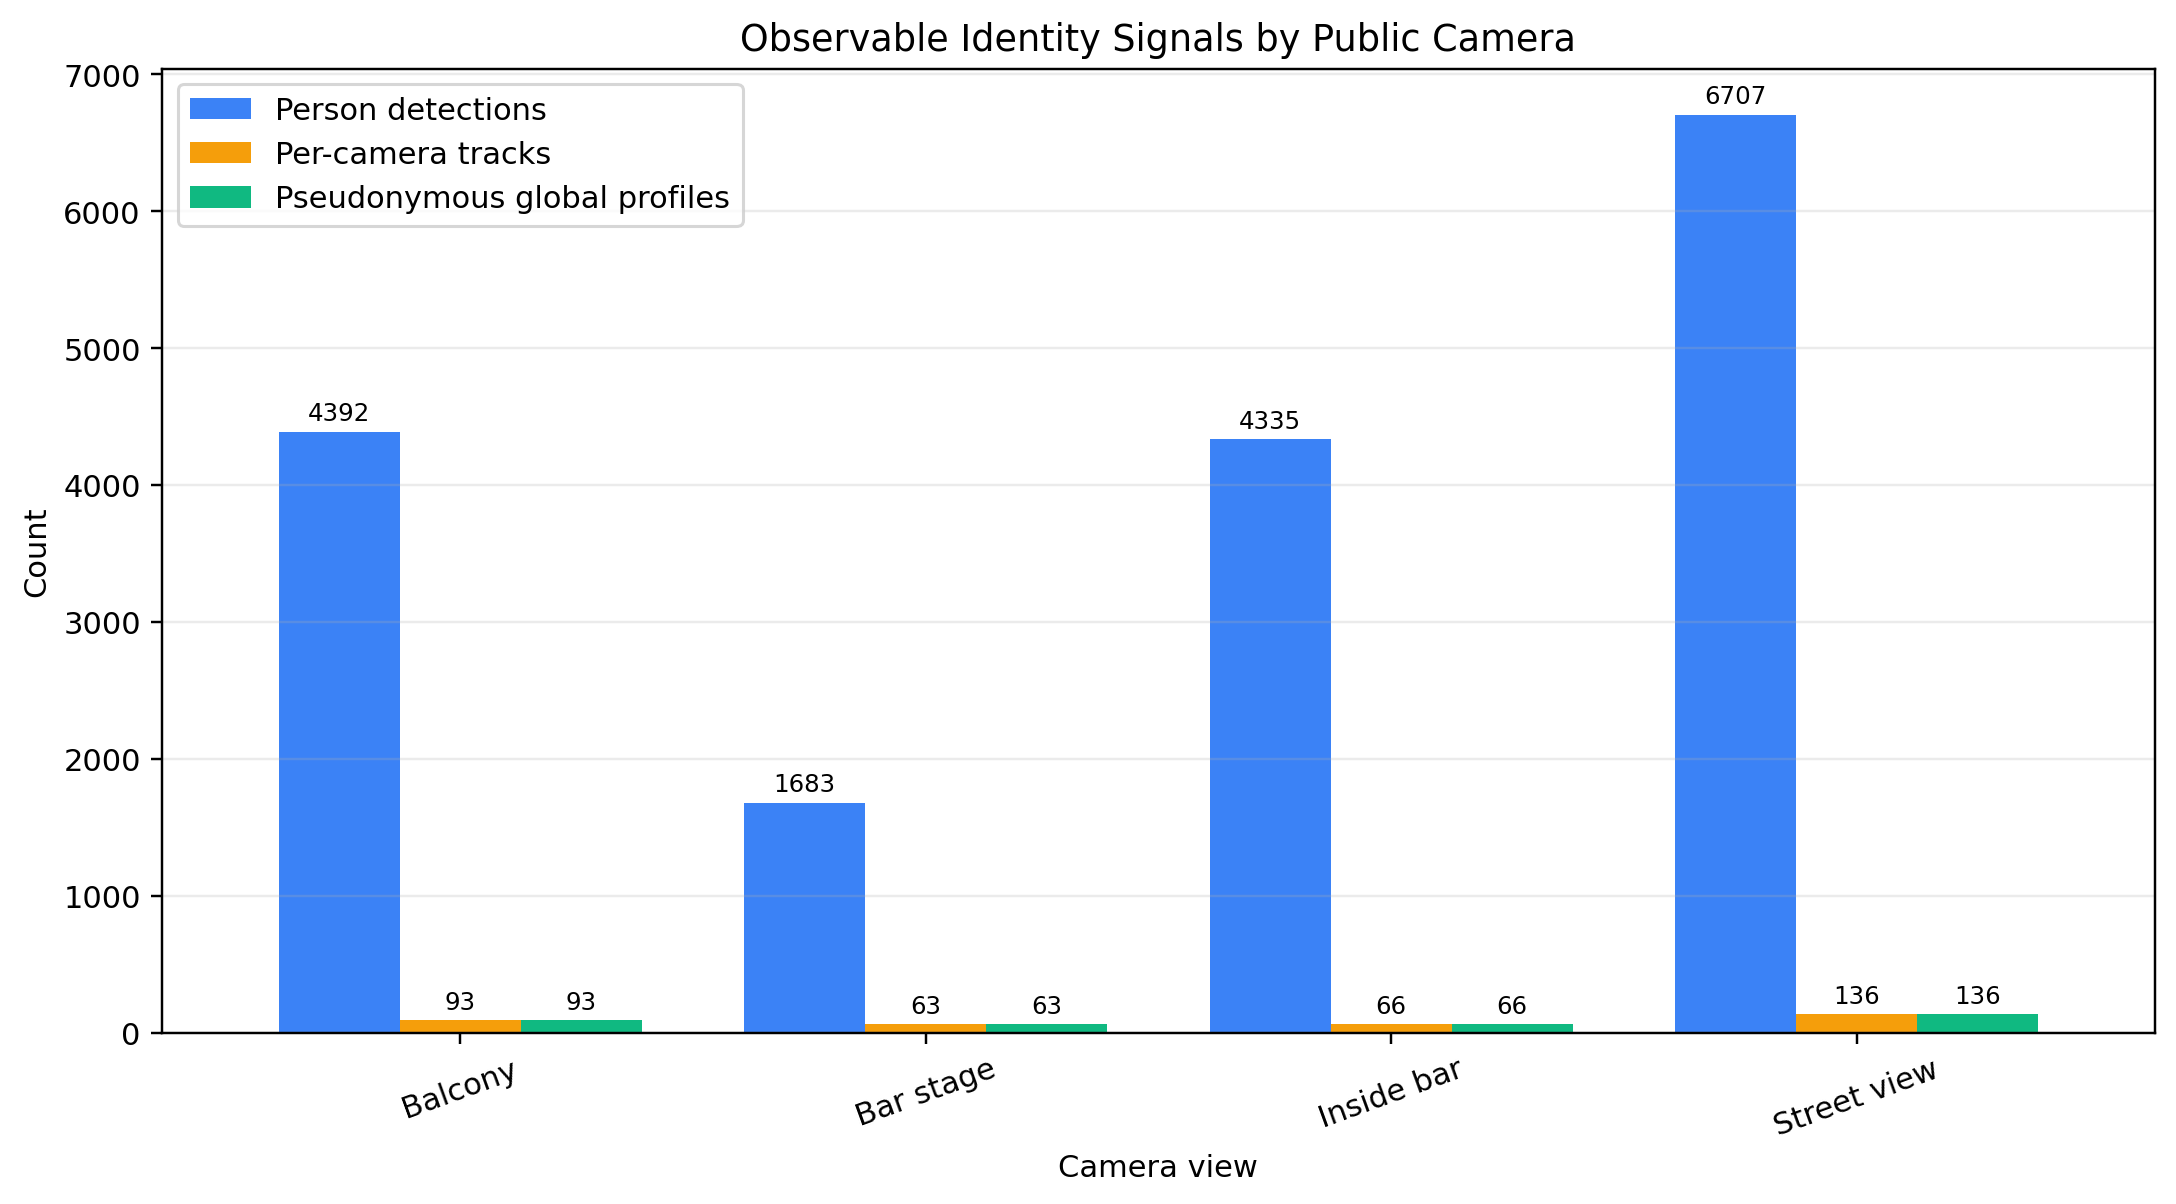
\includegraphics[width=\linewidth]{paper_figures/01_detection_volume_by_camera.png}
    \caption{Person detections, per-camera tracks, and pseudonymous global
    profiles extracted from the four public camera views.}
    \label{fig:detection-volume}
\end{figure}

\subsection{Cross-Camera Profile Linking}
\label{subsec:cross-camera-profile-linking}

Figure~\ref{fig:global-id-span} shows the distribution of global IDs by the
number of camera views in which each ID appeared. Most global IDs appeared in a
single camera view, while seven appeared in more than one camera view. This
finding is directly relevant to the claim because it shows that a subset of
pseudonymous profiles can be linked across public feeds without direct facial
identification.

\begin{figure}[htbp]
    \centering
    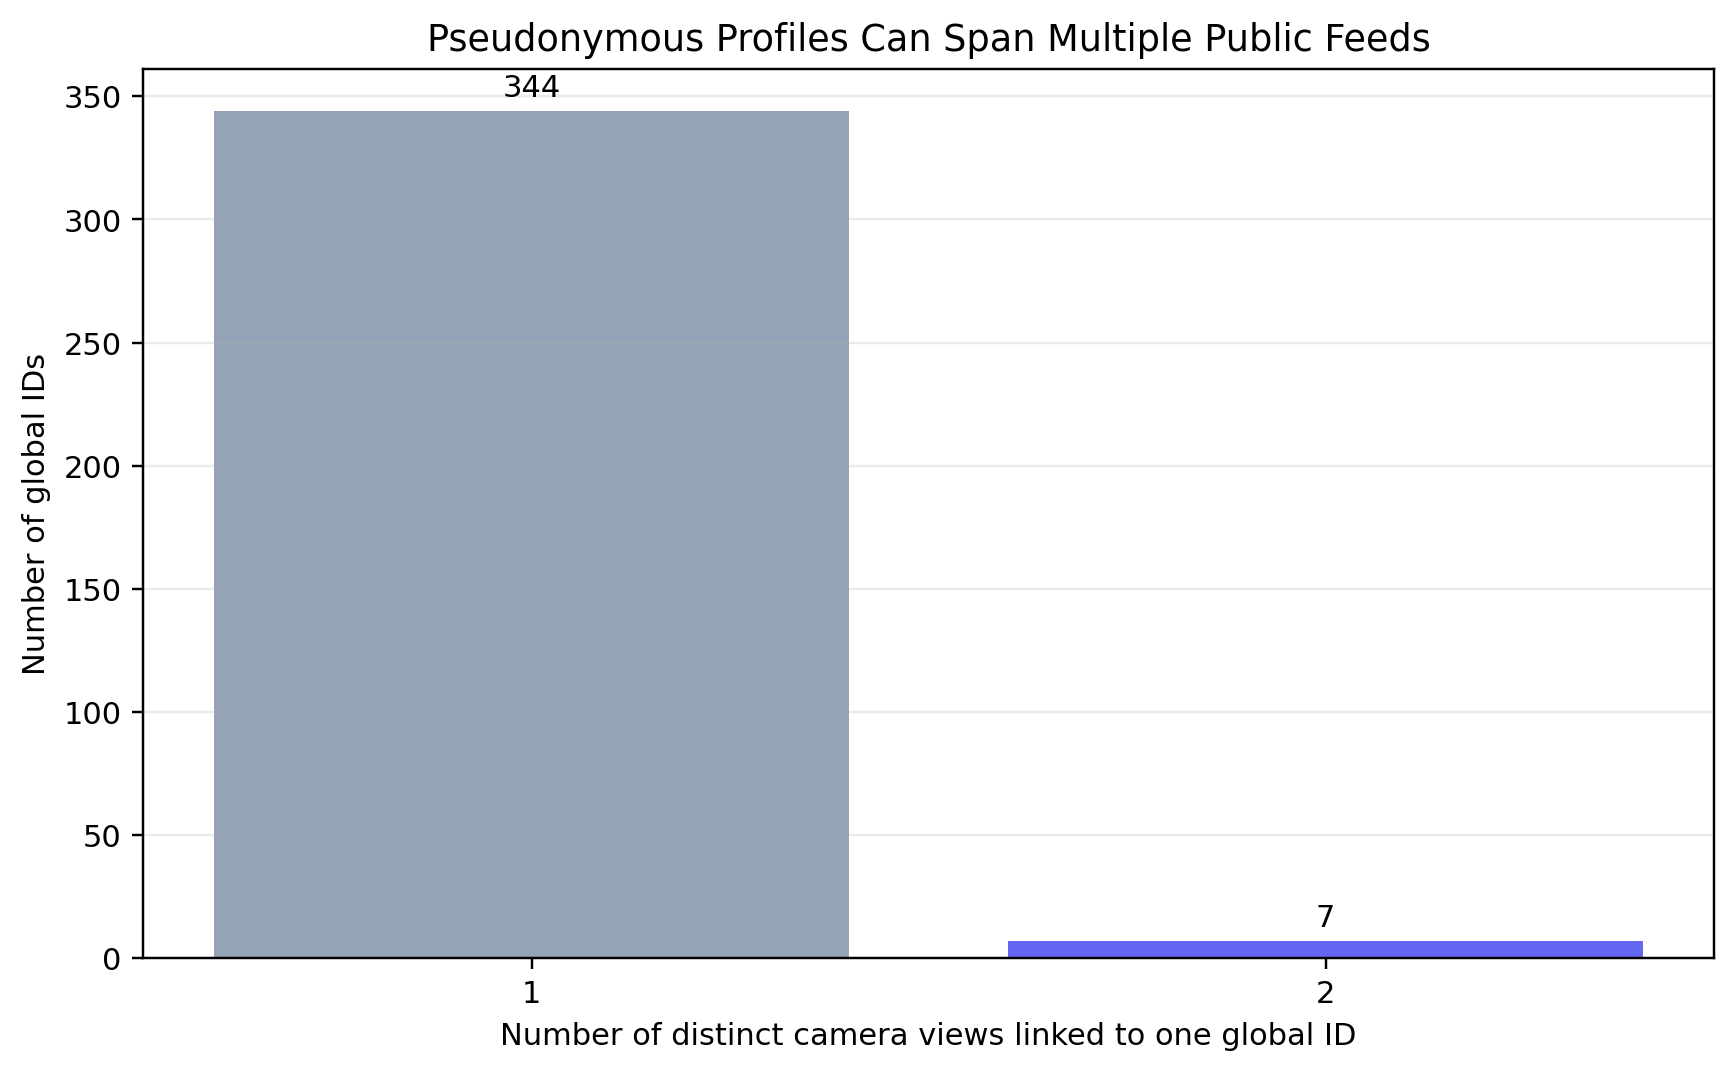
\includegraphics[width=0.82\linewidth]{paper_figures/02_global_ids_by_camera_span.png}
    \caption{Distribution of pseudonymous global IDs by the number of camera
    views in which each profile appeared.}
    \label{fig:global-id-span}
\end{figure}

The top cross-camera profiles were observed across two camera views. The most
persistent cross-camera profile, global ID 23, appeared in 172 detections across
172 frames. Other cross-camera profiles included global ID 108 with 163
detections, global ID 65 with 135 detections, global ID 38 with 54 detections,
global ID 37 with 44 detections, global ID 29 with 35 detections, and global ID
45 with 24 detections. These results indicate that cross-camera persistence was
not universal, but it did occur for multiple profiles in the dataset.

\subsection{Persistence of Pseudonymous Profiles}
\label{subsec:persistence}

Figure~\ref{fig:persistent-profiles} presents the twenty most persistent global
profiles by detection count. Several profiles were observed in hundreds of
frames. The highest-count profiles in this figure are not necessarily
cross-camera profiles; rather, they show that repeated observation within a
single public feed can also create persistent pseudonymous records. Red bars
mark profiles that appeared in more than one camera view.

\begin{figure}[htbp]
    \centering
    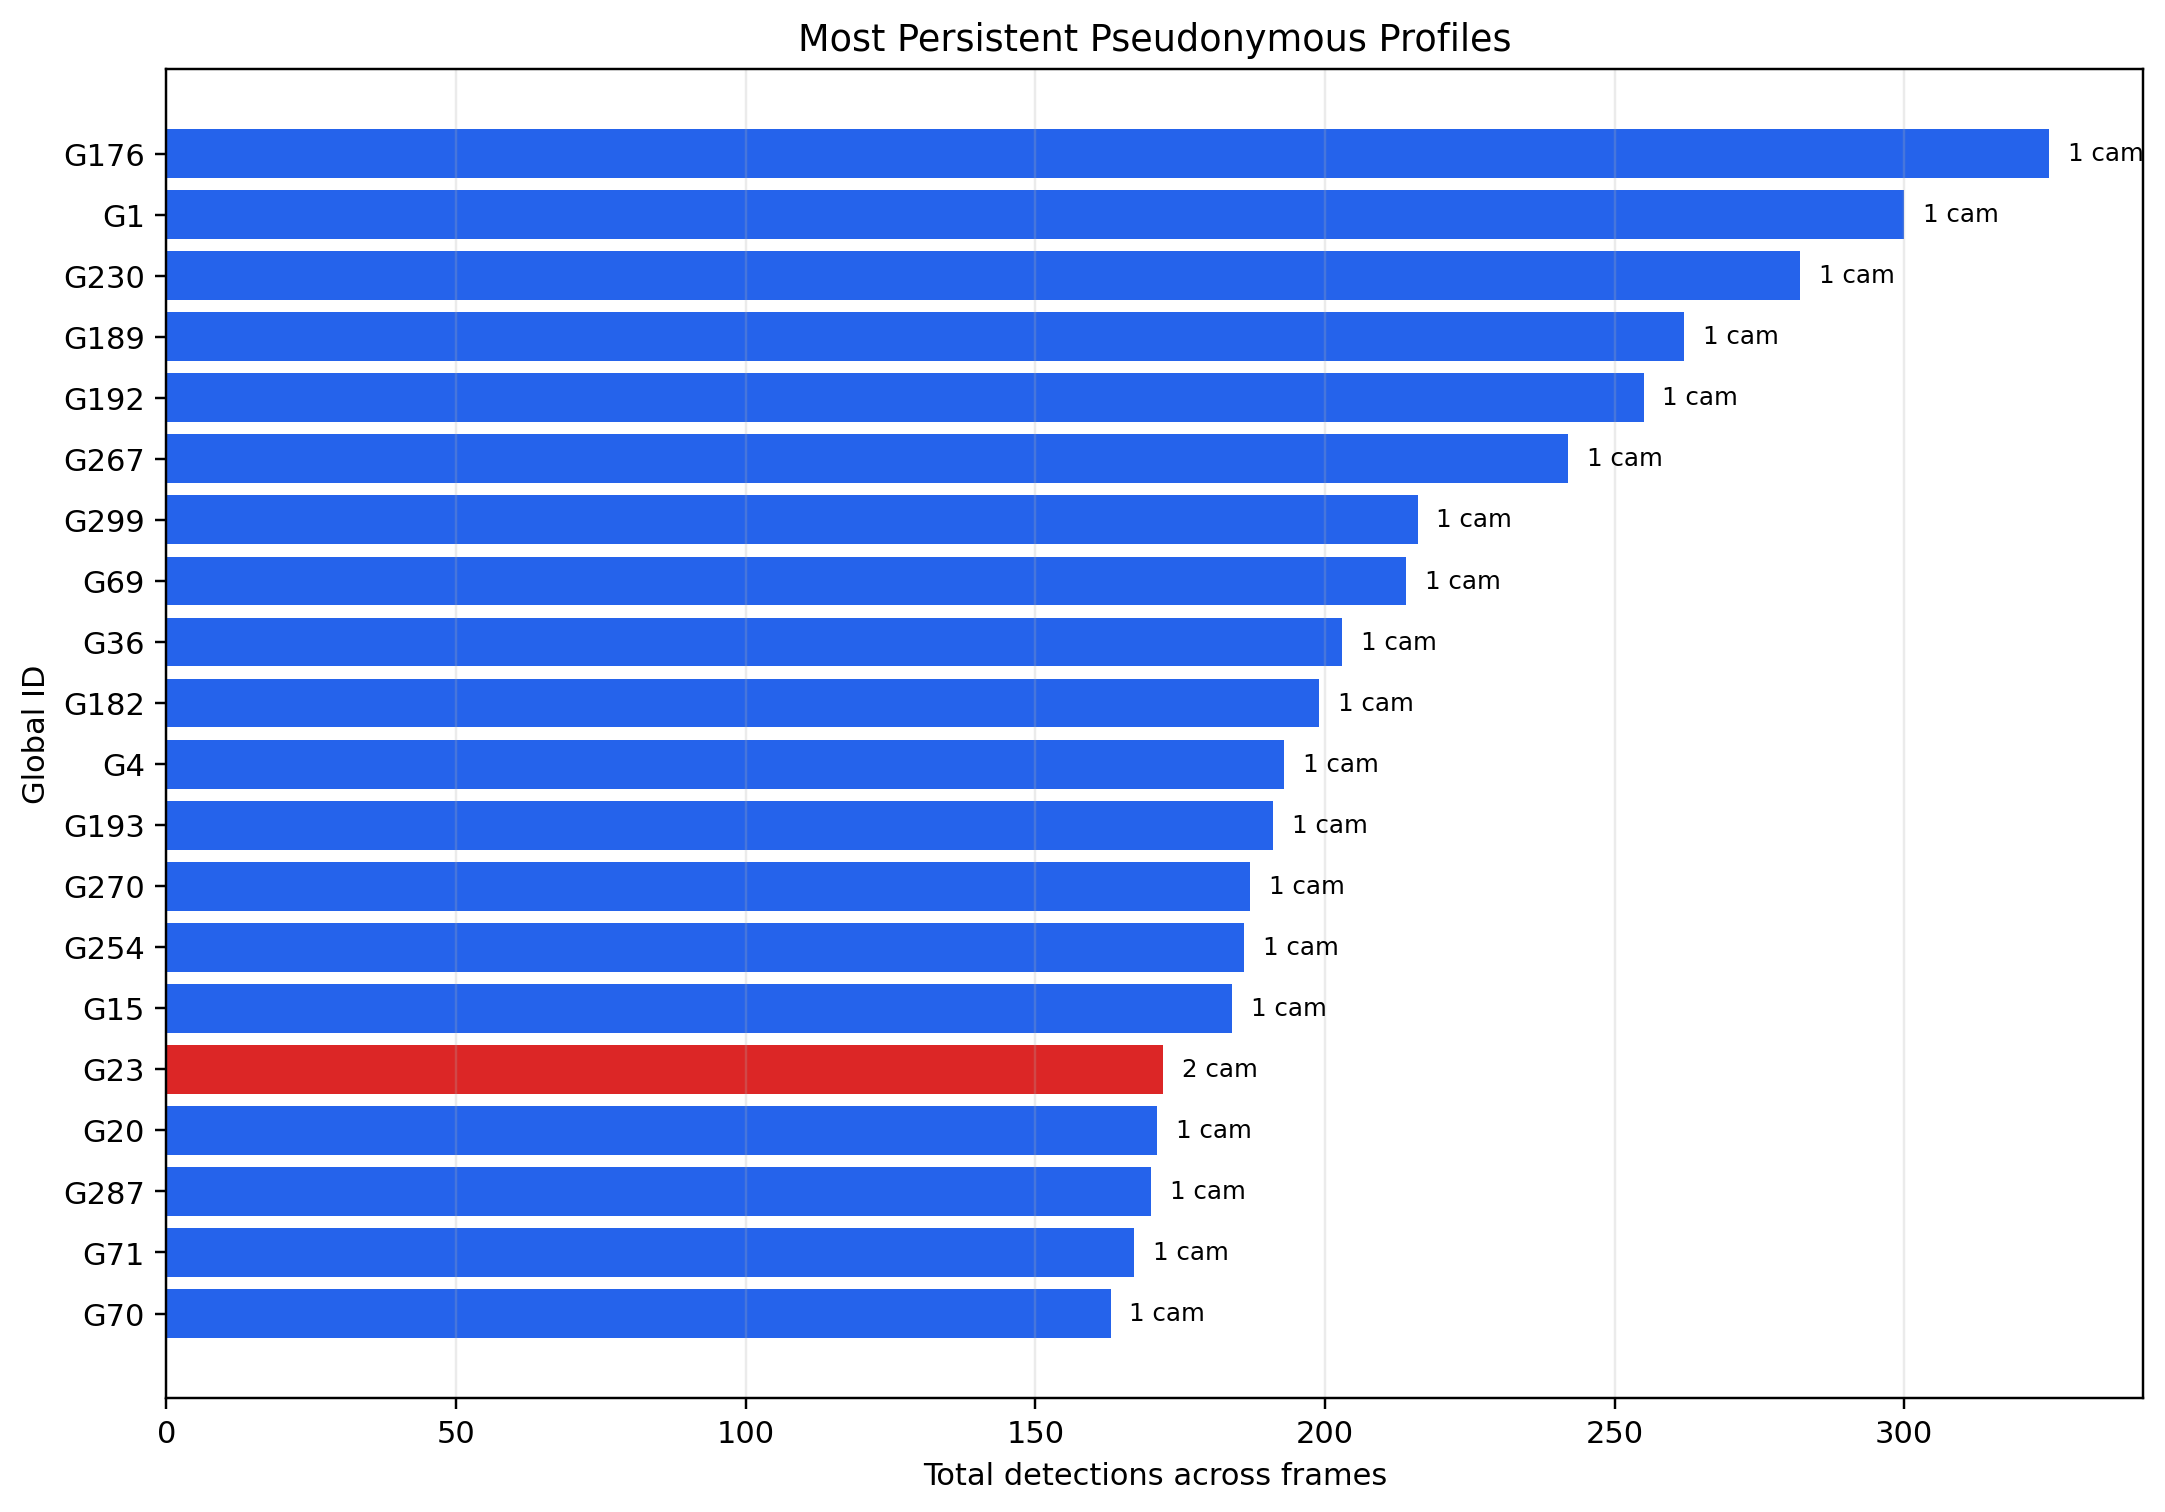
\includegraphics[width=\linewidth]{paper_figures/03_top_persistent_profiles.png}
    \caption{The twenty most persistent pseudonymous profiles by detection
    count. Red bars indicate profiles observed across multiple camera views.}
    \label{fig:persistent-profiles}
\end{figure}

Figure~\ref{fig:profile-timeline} presents a timeline of repeated observations
for frequently detected global IDs. Each point represents one detection in one
frame, colored by camera view. This visualization shows how individual global
IDs accumulate observations over time. For the research question, the important
result is that the pipeline produces temporal traces, not only isolated
detections.

\begin{figure}[htbp]
    \centering
    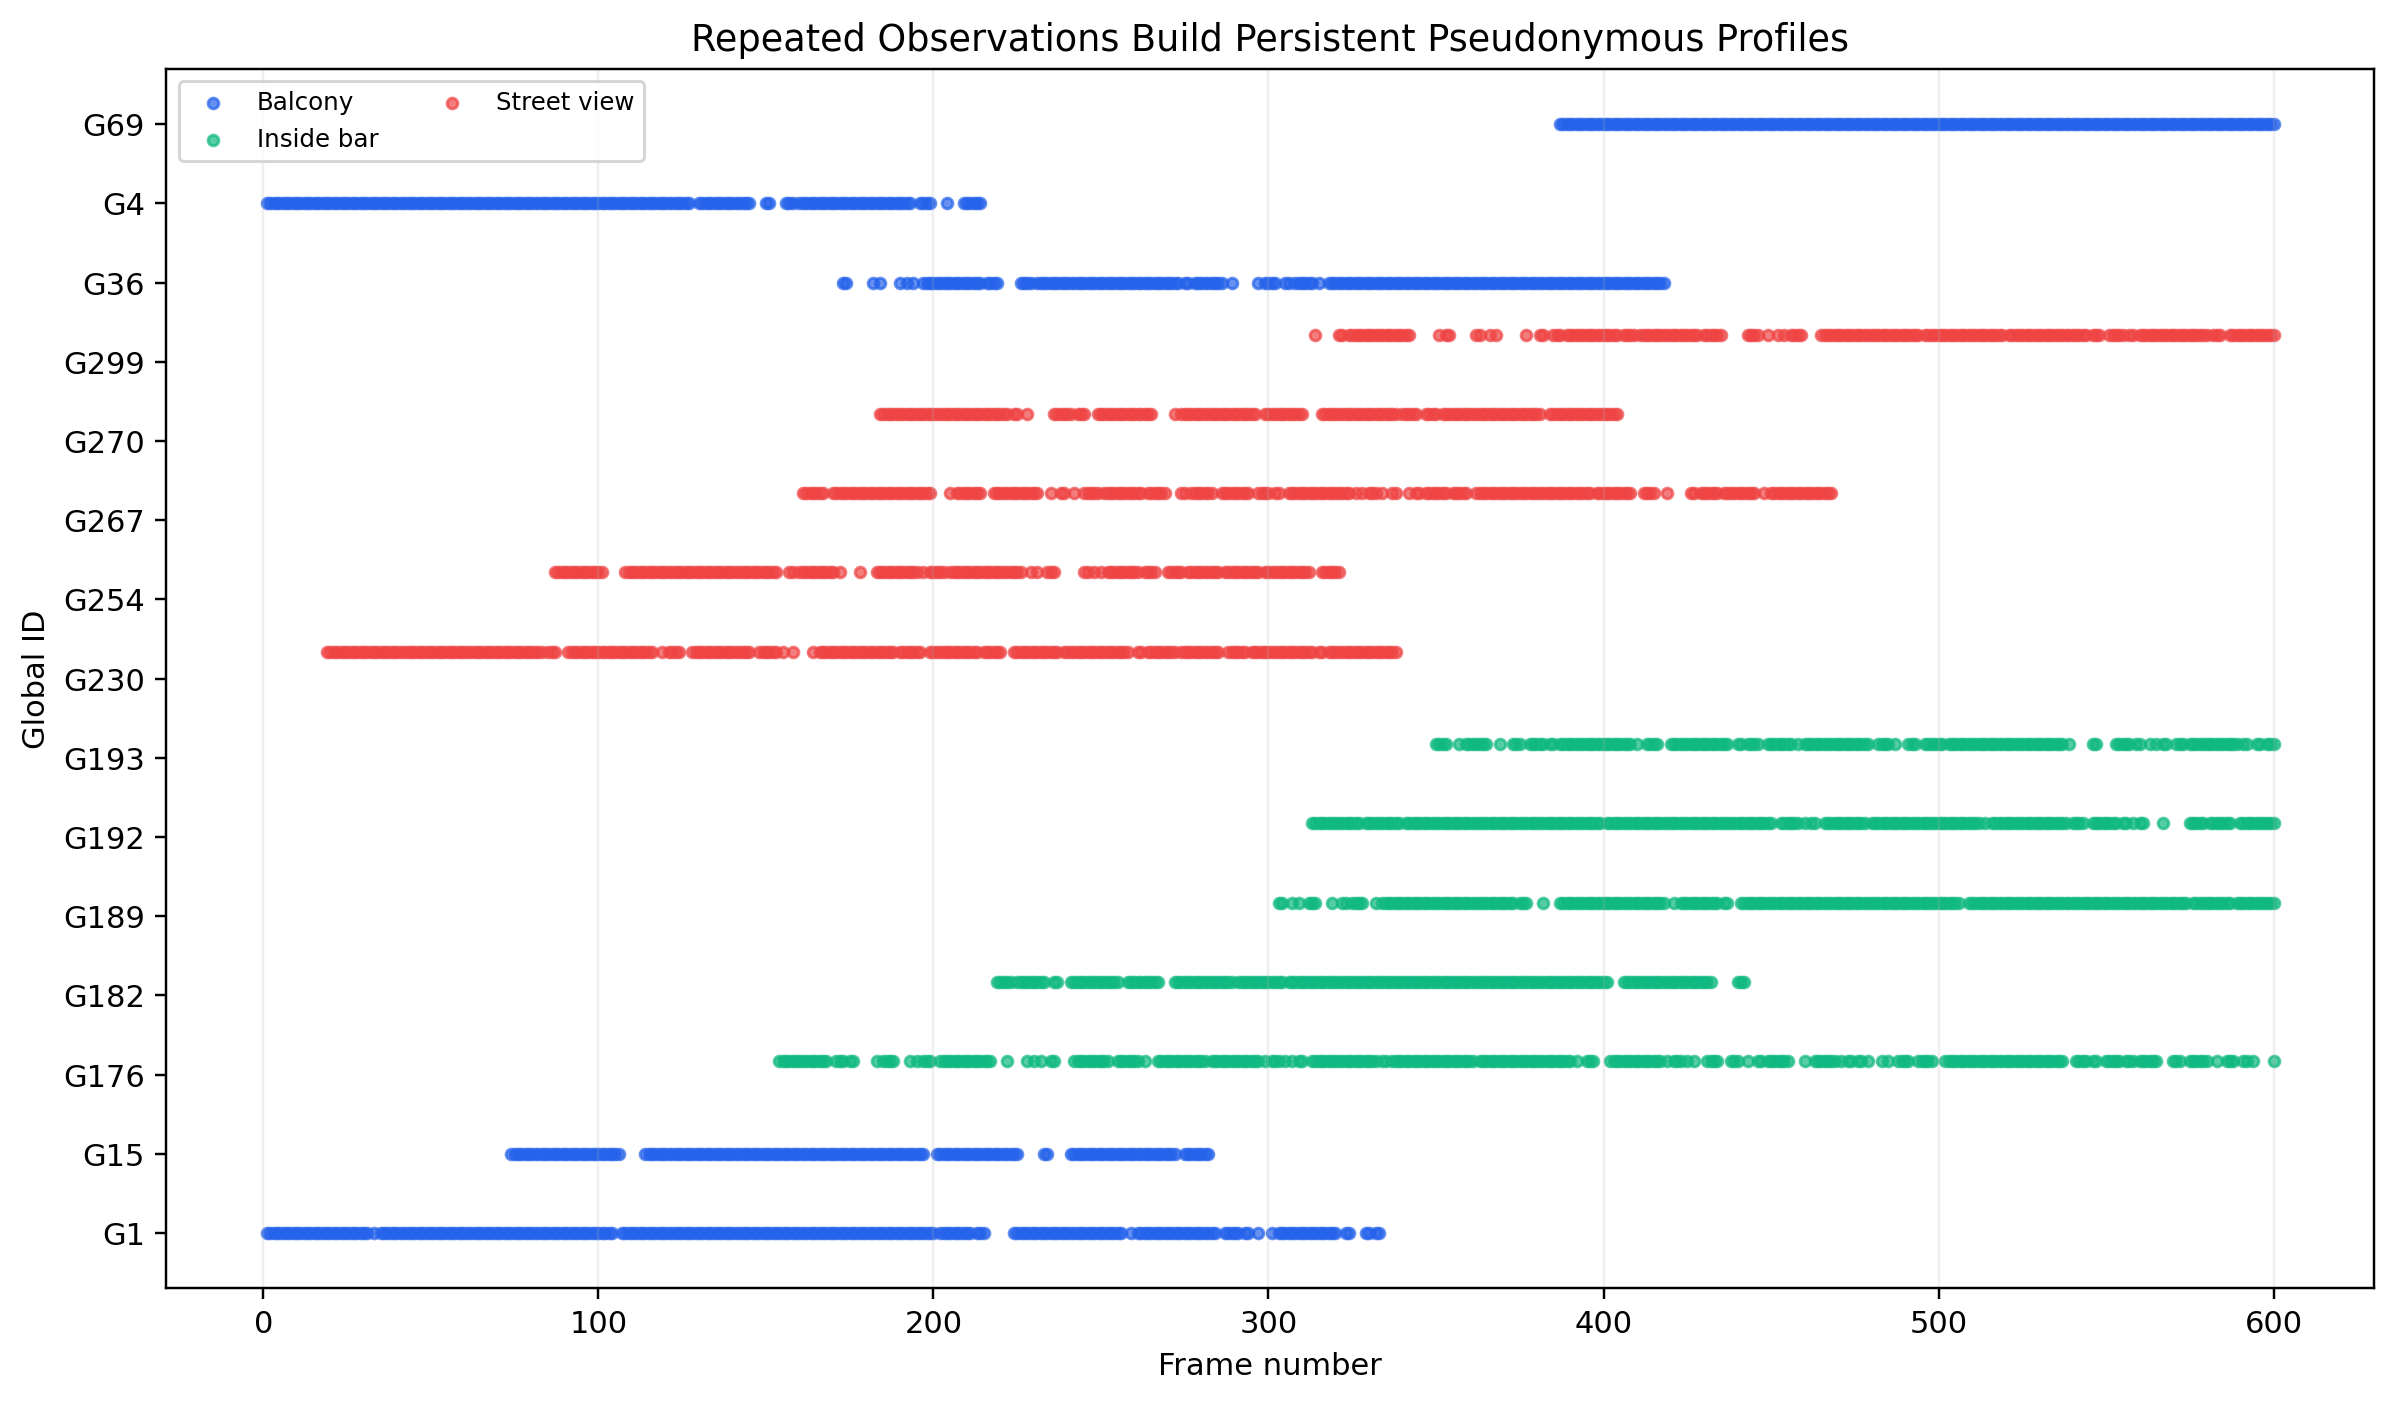
\includegraphics[width=\linewidth]{paper_figures/04_profile_observation_timeline.png}
    \caption{Observation timeline for frequently detected pseudonymous global
    IDs. Each point represents a detection in a frame, colored by camera view.}
    \label{fig:profile-timeline}
\end{figure}

\subsection{Detector Confidence and Match Rates}
\label{subsec:confidence-match-rates}

Figure~\ref{fig:confidence-matches} reports detector confidence by camera view
and the share of detections with cross-camera match scores. The detector
confidence plot summarizes the reliability of the initial person detection
stage, while the cross-camera linkage plot shows that only a small subset of
detections were explicitly linked across views. This distinction is important:
the experiment generated many repeated observations, but cross-camera linking
was limited to a smaller subset of cases.

\begin{figure}[htbp]
    \centering
    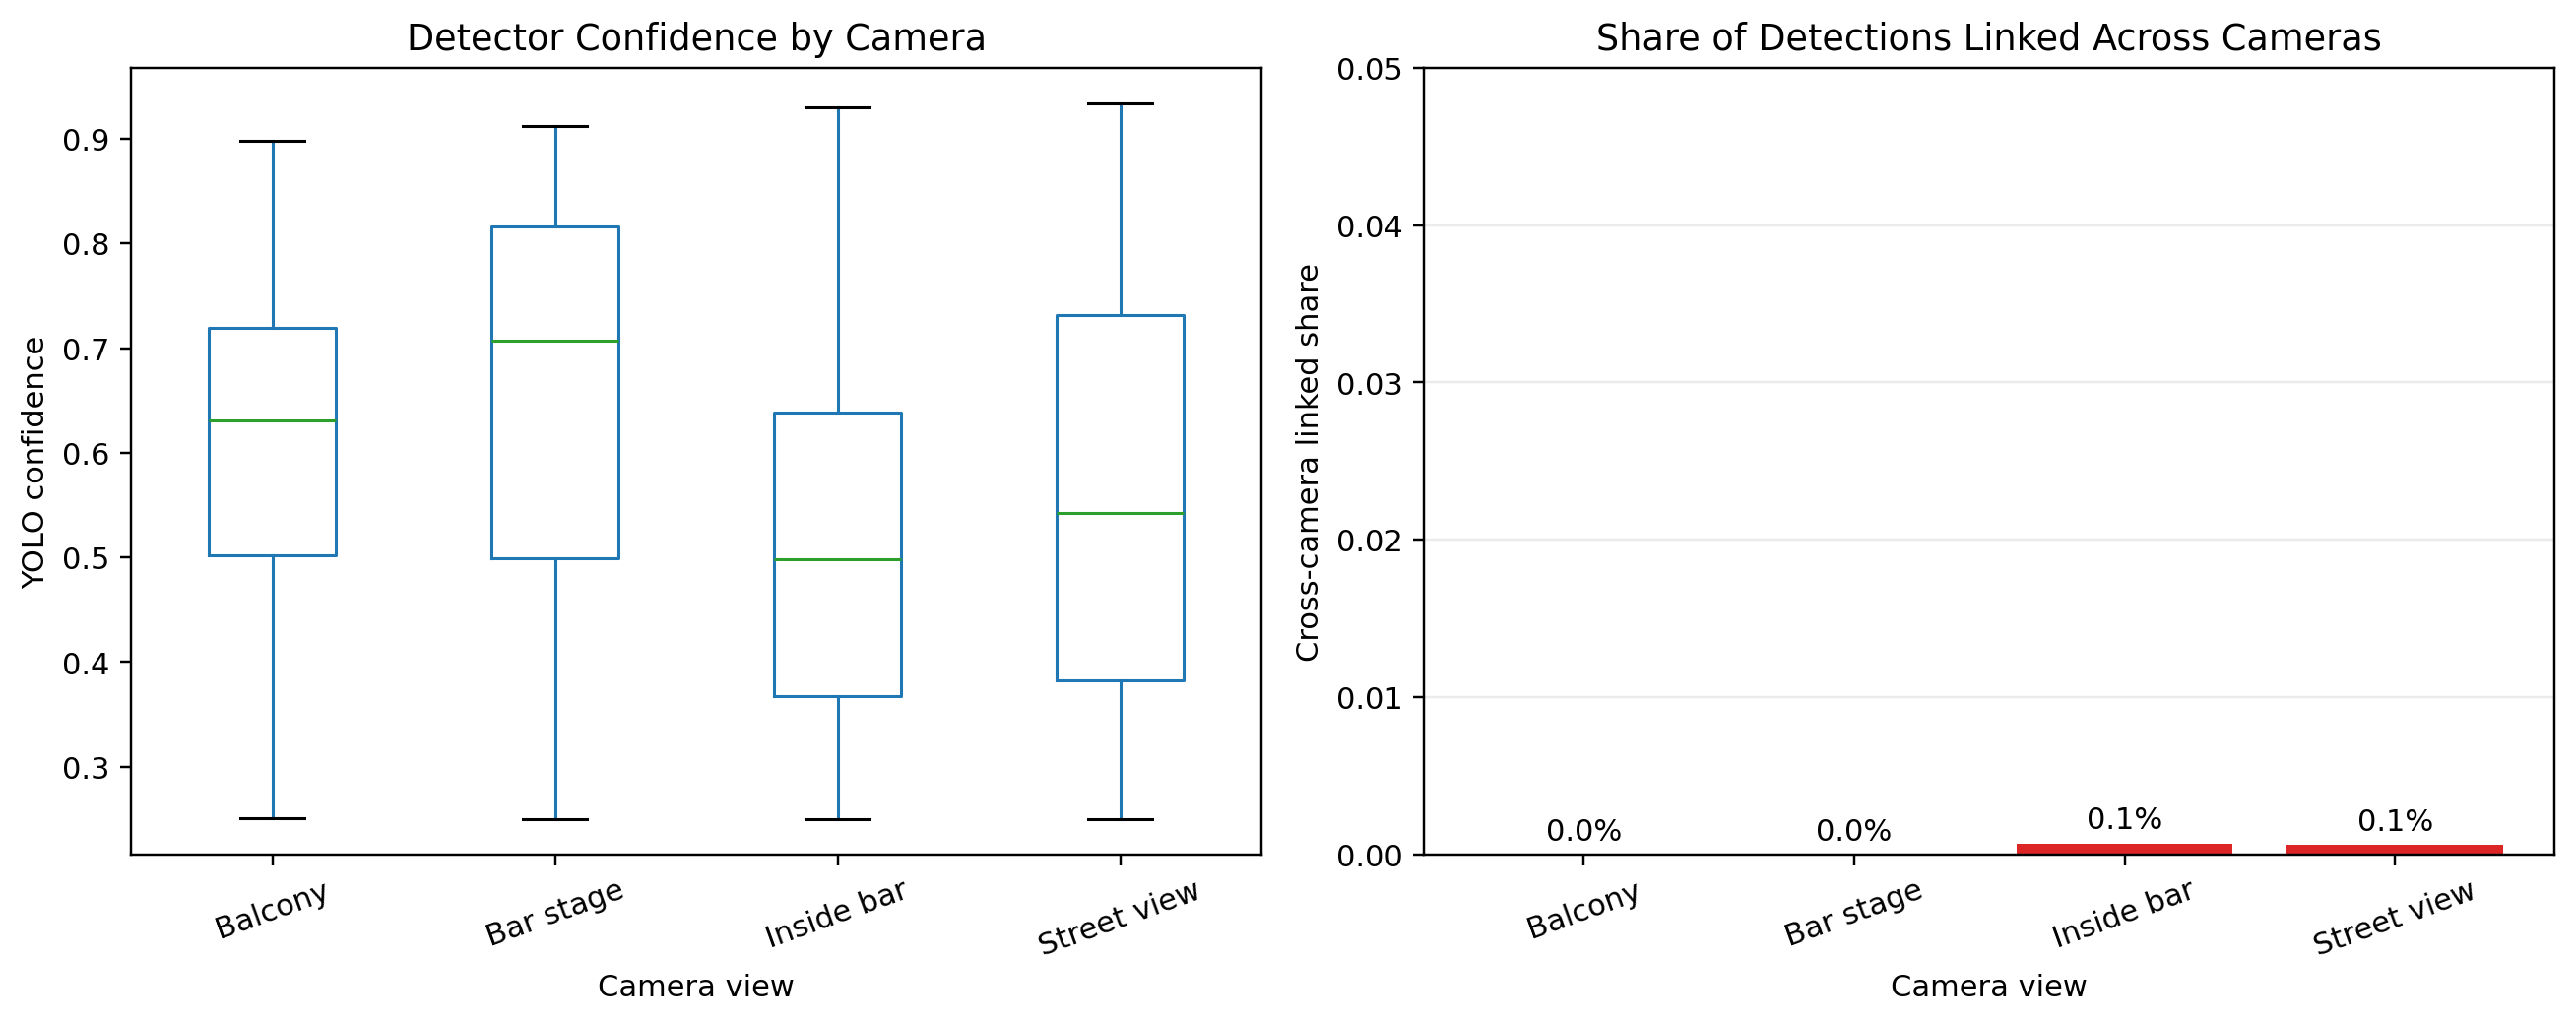
\includegraphics[width=\linewidth]{paper_figures/05_confidence_and_cross_camera_matches.png}
    \caption{Detector confidence and cross-camera linkage rate by camera view.}
    \label{fig:confidence-matches}
\end{figure}

\subsection{Interpretation Relative to the Research Question}
\label{subsec:results-interpretation}

The results show that public camera feeds can be processed into structured
records containing detections, track IDs, global IDs, and temporal observation
patterns. The dataset produced hundreds of local tracks and global pseudonymous
profiles, and a smaller number of profiles were linked across camera views. In
relation to the research question, these findings demonstrate that the relevant
risk is not limited to direct facial identification. Even when the system does
not identify names or faces, repeated public observations can be organized into
persistent pseudonymous profiles.

At the same time, the results also show limitations. Most global profiles were
observed in only one camera view, and the cross-camera match count was small
relative to the total number of detections. The matching method is based on
simple appearance features, so these profile links should be interpreted as
pseudonymous candidates rather than verified identities. These limitations
constrain the strength of the finding but do not remove the observed ability to
produce persistent structured profiles from public video.
